\section{Experiments}
\label{sec:exp}

\subsection{Experimental Setup}

We evaluate RuleDep on seven benchmark datasets that cover both compact and large-scale rule aggregation regimes: KG20C, WN18RR~\cite{dettmers2018convolutional}, Codex-M, FB15k-237~\cite{toutanova2015observed}, Codex-L~\cite{safavi2020codex}, YAGO3-10~\cite{mahdisoltani2014yago3}, and Hetionet~\cite{himmelstein2017hetionet}. These datasets are derived from major knowledge bases including Freebase~\cite{bollacker2008freebase}, WordNet~\cite{miller1995wordnet}, Wikidata~\cite{vrandecic2014wikidata}, YAGO, and Hetionet. All results are reported under the filtered setting using MRR, Hits@1, and Hits@10.

The end-to-end RuleDep workflow consists of three steps. For each dataset, we first mine rules using AnyBURL with a default time budget of 1000\,s, and set a minimum support of 5 for all datasets except the two small ones (KG20C and WN18RR).
\textbf{Step 1 (Rule Learning and Application):} the mined rules are parsed, ranked by confidence, and prefiltered by minimum surprisal; rules are grouped by head atom and applied to the training graph to produce relation-local candidate lists and rule-id tensors for downstream aggregation.
\textbf{Step 2 (Dependency Discovery and Filtering):} for each head atom, we enumerate rule pairs within the group, compute signed lift in failure surprisal space, and apply lift-based and budgeted filtering to retain at most $2\times|\Phi_r|$ dependencies per relation.
\textbf{Step 3 (Relation-Wise Dependency-Aware Aggregation):} we train the linear aggregation model relation by relation on the local candidate sets, using both rule weights and dependency correction terms, and select the best configuration on the validation split.

In practice, RuleDep adopts a relation-wise parameterization rather than a single global rule-identity model. This follows directly from the structure of the rule space: a candidate for relation $r$ can only be supported by rules and dependency edges whose heads predict $r$. Therefore, a single global parameter table would unnecessarily conflate semantically disjoint rule spaces across different target relations. Instead, relation-wise decomposition preserves semantic locality and enables aggressive caching and batched evaluation. Rule application outputs are converted into compact relation-local candidate lists and rule-id tensors, while dependency tensors are loaded only for the active relation. This avoids repeatedly materializing global explanation structures and makes large graphs feasible for dependency-aware training and inference. Peak memory usage is determined by the largest single relation rather than by the entire graph, which is the main scalability advantage of this design.



Table~\ref{tab:exp-datasets} summarizes the size of the datasets together with the size of the induced rule and dependency spaces. The seven datasets differ substantially not only in the number of entities and relations, but also in the density of the dependency space. For example, FB15k-237 has the highest filtered dependency density per rule, while Hetionet has by far the largest absolute number of rules. This heterogeneity is important for our experiments, because it suggests that the best aggregation bias should be dataset dependent rather than universal.

\begin{table}[t]
\centering
\caption{Statistics of the seven datasets and their induced rule and dependency spaces.}
\label{tab:exp-datasets}
\setlength{\tabcolsep}{2.2pt}
\renewcommand{\arraystretch}{1.1}
\footnotesize
\begin{tabular}{lrrrrrrr}
\toprule
Data & Ent. & Rel. & Train & Valid & Test & Rule & Filt.\ dep. \\
\midrule
KG20C      & 16,362   & 5   & 48,213    & 3,670   & 3,724   & 154,790   & 168,315   \\
WN18RR     & 40,943   & 11  & 86,835    & 3,034   & 3,134   & 76,909    & 45,212    \\
Codex-M    & 17,050   & 51  & 185,584   & 10,310  & 10,311  & 518,279   & 883,207   \\
FB15k-237  & 14,541   & 237 & 272,115   & 17,535  & 20,466  & 1,737,378 & 3,946,389 \\
Codex-L    & 77,951   & 69  & 551,193   & 30,622  & 30,622  & 273,472   & 455,330   \\
YAGO3-10   & 123,182  & 37  & 1,079,040 & 5,000   & 5,000   & 990,481   & 1,707,159 \\
Hetionet   & 45,158   & 24  & 1,800,157 & 225,020 & 225,020 & 6,103,910 & 7,154,604 \\
\bottomrule
\end{tabular}
\end{table}

We compare the following families of aggregation methods. First, we include the non-trainable application baselines Max+ and Noisy-OR. Second, we include a canonical supervised baseline that reweights rules without explicit dependency features. Hetionet is excluded from this baseline because the canonical global model terminated with out-of-memory errors. Third, we include the default configuration of RuleDep (RuleDep-default), which applies dependency-aware aggregation without type-level grouping and serves as the main reference point for later ablations. 

In the overall benchmark, RuleDep-best and RuleDep-ensemble denote the best single configuration per dataset and a relation-wise ensemble over all evaluated configurations, respectively. The ensemble selects, for each relation, the best validation configuration according to validation MRR and aggregates the corresponding test results. Unless otherwise stated, all model selection is performed on the validation split. This mirrors the practical use case of RuleDep: the dependency-aware correction is not assumed to be uniformly helpful, but is activated when the validation signal indicates that the extra structural bias is worthwhile. At the same time, the ensemble does not uniformly outperform the best single configuration: on several datasets, the ensemble MRR falls slightly below the best single-config result. This occurs when the validation signal selects configurations that generalize less well to the test split, highlighting the inherent variance of relation-wise model selection.

\subsection{Overall Results and Efficiency}



\begin{table*}[t]
\centering
\caption{Overall benchmark comparison in the style of Ott et al.~\cite{ott_rule-based_2023}. Symbols indicate published results ($^{\dagger}$), AnyBURL with the corresponding aggregator ($^{\star}$), and our current RuleDep pipeline ($^{\diamond}$); blank entries indicate unavailable aligned results.}
\label{tab:overall-results}
\setlength{\tabcolsep}{1.0pt}
\renewcommand{\arraystretch}{1.05}
\footnotesize
\begin{tabular}{ll*{7}{ccc}}
\toprule
\multirow{2}{*}{} & \multirow{2}{*}{Approach} & \multicolumn{3}{c}{KG20C} & \multicolumn{3}{c}{WN18RR} & \multicolumn{3}{c}{\makecell{Codex-\\M}} & \multicolumn{3}{c}{\makecell{FB15k-\\237}} & \multicolumn{3}{c}{\makecell{Codex-\\L}} & \multicolumn{3}{c}{\makecell{YAGO\\3-10}} & \multicolumn{3}{c}{\makecell{Hetio-\\net}} \\
\cmidrule(lr){3-5}\cmidrule(lr){6-8}\cmidrule(lr){9-11}\cmidrule(lr){12-14}\cmidrule(lr){15-17}\cmidrule(lr){18-20}\cmidrule(lr){21-23}
 & & MRR & H@1 & H@10 & MRR & H@1 & H@10 & MRR & H@1 & H@10 & MRR & H@1 & H@10 & MRR & H@1 & H@10 & MRR & H@1 & H@10 & MRR & H@1 & H@10 \\
\midrule
\multirow{13}{*}{\rotatebox{90}{Latent}}
& RESCAL   & .191 & .129 & .308 & .468 & .439 & .521 & .317 & .244 & .456 & \textbf{.357} & .263 & \textbf{.541} & .304 & .242 & .419 & -- & -- & -- & .187 & .106 & .377 \\
& DistMult & .226 & .156 & .367 & .452 & .413 & .531 & .319 & .246 & .458 & .343 & .250 & .531 & .304 & .241 & .423 & .501 & .412 & .661 & -- & -- & -- \\
& ComplEx  & .203 & .140 & .326 & .477 & .438 & .543 & .337 & .262 & .476 & .348 & .253 & .534 & .294 & .237 & .400 & \underline{.576} & \underline{.505} & .704 & .250 & .152 & .470 \\
& ConvE    & .171 & .109 & .291 & .447 & .411 & .508 & .318 & .239 & .464 & .339 & .248 & .521 & .303 & .240 & .420 & .488 & .399 & .657 & .180 & .100 & .318 \\
& RotatE   & .212 & .133 & .362 & .475 & .426 & .574 & .305 & .224 & .454 & .336 & .238 & .531 & .250 & .177 & .389 & .498 & .405 & .670 & .257 & .185 & .403 \\
& TuckER   & .177 & .119 & .295 & .459 & .430 & .514 & .328 & .259 & .458 & .352 & .259 & \underline{.536} & .309 & .244 & .430 & .544 & .465 & .680 & -- & -- & -- \\
\cmidrule(l){2-23}
& CompGCN  & -- & -- & -- & .479 & .443 & .546 & -- & -- & -- & .355 & .264 & .535 & -- & -- & -- & .421 & .392 & .577 & -- & -- & -- \\
& NBFNet   & -- & -- & -- & .551 & .497 & .666 & -- & -- & -- & .415 & .321 & .599 & -- & -- & -- & .550 & .479 & .686 & -- & -- & -- \\
& AdaProp  & -- & -- & -- & \underline{.562} & \underline{.499} & \underline{.671} & -- & -- & -- & .417 & .331 & .585 & -- & -- & -- & .573 & .510 & .685 & -- & -- & -- \\
& DRUM$^{\dagger}$      & -- & -- & -- & .486 & .425 & .586 & -- & -- & -- & .343 & .255 & .516 & -- & -- & -- & -- & -- & -- & -- & -- & -- \\
& Neural LP$^{\dagger}$ & -- & -- & -- & .435 & .371 & .566 & -- & -- & -- & .240 & -- & .362 & -- & -- & -- & -- & -- & -- & -- & -- & -- \\
& RNNLogic & -- & -- & -- & .483 & .446 & .558 & -- & -- & -- & .344 & .252 & .530 & -- & -- & -- & .554 & .509 & .622 & -- & -- & -- \\
& Dense$^{\star}$ & -- & -- & -- & \underline{.507} & \underline{.466} & \underline{.587} & .331 & .261 & .465 & .335 & .245 & .510 & -- & -- & -- & -- & -- & -- & -- & -- & -- \\
\midrule
\multirow{12}{*}{\rotatebox{90}{Interpretable}}
& GPFL$^{\dagger}$      & -- & -- & -- & .480 & .449 & .552 & -- & -- & -- & .322 & .247 & .504 & -- & -- & -- & -- & -- & -- & -- & -- & -- \\
& AMIE3$^{\dagger}$     & -- & -- & -- & .450 & .419 & .514 & .263 & .198 & .395 & .247 & .178 & .394 & .026 & -- & .029 & .250 & .206 & .343 & -- & -- & -- \\
& RuleN$^{\dagger}$     & -- & -- & -- & -- & .427 & .536 & -- & -- & -- & -- & .182 & .420 & -- & -- & -- & -- & -- & -- & -- & -- & -- \\
& C-NN$^{\dagger}$      & -- & -- & -- & .469 & .444 & .519 & -- & -- & -- & .296 & .222 & .446 & -- & -- & -- & .512 & .424 & .678 & -- & -- & -- \\
\cmidrule(l){2-23}
& Max+$^{\star}$      & .215 & .143 & .361 & .497 & .458 & .574 & .319 & .249 & .455 & .329 & .245 & .503 & .311 & .254 & .425 & .554 & .487 & .679 & .351 & .292 & .467 \\
& Noisy-OR$^{\star}$  & .230 & .157 & \underline{.376} & .459 & .407 & .567 & .301 & .226 & .448 & .338 & .252 & .507 & .303 & .242 & .424 & .530 & .450 & .675 & .303 & .240 & .432 \\
& Sparse$^{\star}$    & -- & -- & -- & .499 & .459 & .574 & .335 & .266 & .467 & .352 & .266 & .526 & -- & -- & -- & -- & -- & -- & -- & -- & -- \\
& SAFRAN$^{\star}$    & -- & -- & -- & .502 & .459 & .578 & .320 & .253 & .449 & .351 & \underline{.269} & .513 & -- & -- & -- & -- & -- & -- & -- & -- & -- \\
% & Canonical$^{\star}$ & .239 & .166 & .376 & .500 & .456 & .584 & .346 & .277 & .481 & .354 & .267 & .530 & -- & -- & -- & .574 & .501 & .703 & -- & -- & -- \\
& Canonical$^{\diamond}$ & .228 & .155 & .368 & .499 & .455 & .584 & .341 & .272 & .475 & .345 & .259 & .518 & .330 & .271 & .444 & .572 & .500 & .704 & -- & -- & -- \\
\cmidrule(l){2-23}
& RuleDep-default$^{\diamond}$      & \underline{.233} & \underline{.160} & .371 & \underline{.501} & .457 & \underline{.584} & .342 & .273 & \textbf{.479} & .348 & .262 & .518 & .334 & .274 & \underline{.448} & .575 & \underline{.503} & \underline{.706} & .362 & .300 & .484 \\
& RuleDep-best$^{\diamond}$ & \underline{.233} & \textbf{.161} & .374 & \textbf{.502} & \textbf{.460} & .583 & \underline{.344} & \underline{.276} & \underline{.478} & \underline{.354} & \underline{.265} & \textbf{.530} & \underline{.334} & \underline{.275} & \underline{.448} & \underline{.576} & \textbf{.504} & \underline{.705} & \underline{.374} & \underline{.314} & \underline{.496} \\
& RuleDep-ensemble$^{\diamond}$ & \textbf{.235} & \textbf{.161} & \textbf{.378} & .500 & .456 & \textbf{.585} & \textbf{.346} & \textbf{.278} & \textbf{.479} & \textbf{.357} & \textbf{.271} & \textbf{.530} & \textbf{.335} & \textbf{.276} & \textbf{.450} & \textbf{.577} & \textbf{.504} & \textbf{.707} & \textbf{.380} & \textbf{.318} & \textbf{.505} \\
\bottomrule
\end{tabular}
\end{table*}

All latent-model results in Table~\ref{tab:overall-results} are taken from official LibKGE/CoDEx benchmark results. For FB15k-237, WN18RR, and Codex-M, we retain the published numbers of prior methods. For the four additional datasets, only methods available in our evaluation are reported. Three observations stand out. First, the classical baselines already show that strong performance can be achieved with interpretable rule aggregation, especially on WN18RR and FB15k-237. Second, the extended RuleDep evaluation improves over the default setting on the larger and more heterogeneous datasets: the RuleDep family as a whole leads the majority of dataset-metric cells in the table, while the canonical baseline captures a small number of cells on KG20C and H@10-dominant metrics. Third, relation-wise model selection matters most on heterogeneous datasets: the gap between RuleDep-best and RuleDep-ensemble is smallest on YAGO3-10 and Codex-L, but remains clearly visible on FB15k-237 and Hetionet.

The benchmark table also makes the central trade-off of RuleDep more visible. On the three standard datasets shared with prior work, the RuleDep-default configuration and its stronger best or ensemble variants remain competitive with the strongest interpretable baselines, while the Canonical baseline reproduction remains a strong rule-only reference point. This supports the interpretation that canonical aggregation already captures most marginal rule effects. RuleDep adds a smaller but still useful dependency-aware correction on top of that. On the four additional datasets, the new Max+/Noisy-OR rows establish strong application baselines, while the RuleDep-default rows show that the dependency-aware correction remains beneficial beyond the classic three-dataset benchmark.

The accuracy gains in Table~\ref{tab:overall-results} must be read together with training cost. In several datasets, the canonical global model remains a very strong rule-only baseline, which confirms that most predictive signal is already contained in reweighted individual rules. However, the global training regime is substantially more expensive. Figure~\ref{fig:runtime-global-vs-ruledep} visualizes this trade-off for six datasets. Hetionet is excluded because the canonical run terminated with out-of-memory errors before producing a comparable wall-clock result.

\begin{figure}[t]
\centering
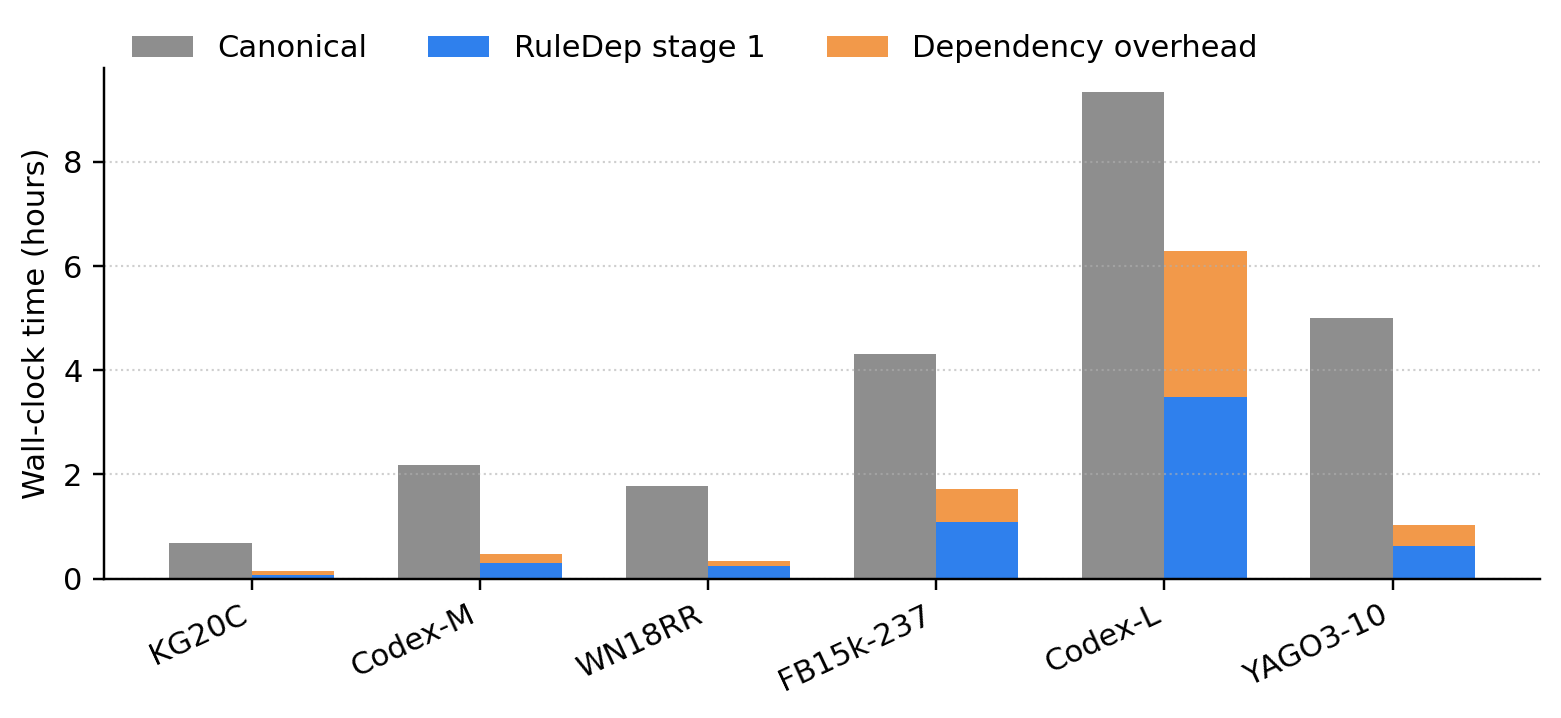
\includegraphics[width=\linewidth]{pic/runtime_canonical_vs_ruledep}
\caption{Wall-clock comparison between the global canonical baseline and the best RuleDep configuration on six datasets. The gray bar is the total runtime of the canonical global model. The RuleDep bar is decomposed into the relation-wise canonical baseline sweep (blue) and the additional dependency training overhead (orange). Hetionet is excluded because the canonical run terminated with out-of-memory errors.}
% \Description{...} % removed for IEEE format
\label{fig:runtime-global-vs-ruledep}
\end{figure}

A similar pattern emerges when we compare against the learned Dense and Sparse aggregators reported by Ott et al.~\cite{ott_rule-based_2023}: their canonical logistic baseline is already competitive in accuracy, but the latent aggregators are much more expensive. On FB15k-237 and WN18RR, their logistic model trains $27\times$/$39\times$ faster than Dense and $4.8\times$/$7.3\times$ faster than Sparse. Our results extend this efficiency argument from the global rule-only setting to the dependency-aware setting: RuleDep sacrifices some of the accuracy of a single global model on several datasets, but in return it keeps training tractable on datasets where a global dependency-aware model would be prohibitively expensive.

\subsection{When Does Dependency Help?}


\begin{table}[t]
\centering
\caption{Representative relation-level gains from RuleDep. Each dataset shows the two relations with the highest relative MRR gain over the canonical baseline; DrD and DpS denote ``Disease resembles Disease'' and ``Disease presents Symptom''.}
\label{tab:relation-positive-cases}
\setlength{\tabcolsep}{3pt}
\renewcommand{\arraystretch}{1.05}
\footnotesize
\begin{tabular}{llrrrrr}
\toprule
Dataset & Relation & \makecell{Avg\\Obj.} & \makecell{Avg\\Subj.} & Canon. & RuleDep & \makecell{Rel.\\Gain} \\
\midrule
\multirow{2}{*}{KG20C} & author\_write\_paper & 1.54 & 2.52 & .231 & .248 & 7.5\% \\
 & paper\_in\_domain & 3.61 & 9.24 & .116 & .118 & 1.5\% \\
\multirow{2}{*}{WN18RR} & \_has\_part & 2.43 & 1.21 & .205 & .219 & 6.9\% \\
 & \_member\_meronym & 2.39 & 1.01 & .318 & .329 & 3.4\% \\
\multirow{2}{*}{Codex-M} & P20 (place of death) & 1.00 & 13.17 & .327 & .336 & 2.6\% \\
 & P737 (influenced by) & 2.82 & 2.47 & .119 & .121 & 2.3\% \\
\multirow{2}{*}{FB15k-237} & combatants & 9.11 & 8.59 & .255 & .325 & 27.5\% \\
 & region & 1.17 & 7.48 & .573 & .657 & 14.8\% \\
\multirow{2}{*}{Codex-L} & P749 (parent org.) & 1.07 & 2.64 & .275 & .293 & 6.6\% \\
 & P737 (influenced by) & 2.58 & 2.29 & .114 & .119 & 4.8\% \\
\multirow{2}{*}{YAGO3-10} & dealsWith & 5.92 & 7.75 & .265 & .325 & 22.8\% \\
 & diedIn & 1.00 & 4.89 & .180 & .201 & 11.5\% \\
\multirow{2}{*}{Hetionet} & DrD & 4.11 & 4.27 & .263 & .309 & 17.7\% \\
 & DpS & 20.35 & 6.52 & .233 & .241 & 3.5\% \\
\bottomrule
\end{tabular}
\end{table}

% \begin{figure*}[t]
% \centering
% \includegraphics[width=0.48\textwidth]{pic/exp_gain_vs_stage1}
% \hfill
% \includegraphics[width=0.48\textwidth]{pic/exp_gain_vs_dep_density}
% \caption{Relation-level conditions under which dependency-aware aggregation helps. Left: relative gain versus canonical baseline MRR. Right: relative gain versus dependency density.}
% \Description{Two scatter plots. The left plot compares relation-level relative gain against canonical baseline MRR and shows that higher gains tend to occur on less saturated relations. The right plot compares relative gain against dependency density and shows that gains are more common when more dependencies are available per rule.}
% \label{fig:relation-gain-patterns}
% \end{figure*}

The average gains in Table~\ref{tab:overall-results} hide a much stronger relation-level pattern. Across all $430$ evaluated relations, $95$ relations obtain more than $3\%$ relative MRR gain over the canonical baseline, $218$ relations fall into a stable $0$--$3\%$ gain range, and $131$ relations show negative transfer. RuleDep is therefore not a uniformly strong bias, but a selective correction that is useful when the structural conditions are right.

The strongest relation-level gains are substantial: they reach $27.5\%$ on FB15k-237, $22.8\%$ on YAGO3-10, and $17.7\%$ on Hetionet. At the same time, the positive cases are not confined to one dataset family. KG20C and WN18RR show modest but consistent gains on compact structural relations, while Codex-M and Codex-L still contain clear positive cases even when only a few high-precision dependencies survive filtering.

Two trends are especially consistent. First, positive-gain relations are typically not yet saturated under the canonical baseline: their average canonical baseline MRR is $0.296$, lower than the $0.406$ observed for negative-gain relations. Second, negative-gain relations actually have higher dependency density on average ($1.53$ dependencies per rule vs.~$1.27$ for positive-gain relations), which suggests that raw dependency count alone does not predict benefit---it is the quality and structural alignment of dependencies, rather than their sheer number, that determines whether the correction helps.

The representative relations in Table~\ref{tab:relation-positive-cases} also reveal a clear semantic pattern. FB15k-237 and YAGO3-10 are dominated by event-participation, role-filling, and contextual relations such as \textit{combatants}, \textit{region}, \textit{dealsWith}, and \textit{diedIn}; in these cases, several partially informative rules must co-occur before a candidate becomes convincing. Hetionet shows the same phenomenon in biomedical form: DrD and DpS benefit because disease-level predictions are naturally supported by multiple corroborating biological paths. By contrast, the Codex datasets contain smaller but still consistent gains on attribute-like relations such as P20, P737, and P749, where only a few dependencies survive filtering but still improve ranking. KG20C and WN18RR lie between these extremes: their positive cases are fewer, but the gains are still concentrated on relations where multiple structural cues agree on the same answer. Overall, dependency helps most when relation semantics make co-support meaningful rather than accidental.


\subsection{Ablation and Variant Comparison}



\begin{table}[t]
\centering
\caption{Ablation results across seven datasets (MRR). Rows are grouped as Group A--E by source polarity, core mechanism, initialization/regularization, typed structure, and filtering/budget choices; blank entries indicate unavailable runs.}
\label{tab:ablation-summary}
\setlength{\tabcolsep}{3pt}
\renewcommand{\arraystretch}{1.05}
\footnotesize
\begin{tabular}{l l *{7}{c} c}
\toprule
 & Approach & \makecell{KG\\20C} & \makecell{WN\\18RR} & \makecell{Codex\\-M} & \makecell{FB15k\\-237} & \makecell{Codex\\-L} & \makecell{YAGO\\3-10} & \makecell{Hetio\\-net} & Avg \\
\midrule
\multirow{3}{*}{\rotatebox{90}{Group A}}
& default          & .233 & .501 & .342 & .348 & .334 & .575 & .362 & .385 \\
& w/o synergy      & .230 & .499 & .342 & .347 & .333 & .575 & .362 & .384 \\
& w/o redundancy   & .233 & .500 & .341 & .348 & .333 & .575 & .363 & .385 \\
\midrule
\multirow{3}{*}{\rotatebox{90}{Group B}}
& fix-lift         & .212 & .471 & .315 & .318 & .308 & .525 & .335 & .355 \\
& random-init      & \textbf{.234} & .501 & .338 & .331 & .333 & .569 & .357 & .380 \\
& surprisal-func   & .232 & .499 & .342 & .350 & .333 & .578 & .378 & \textbf{.387} \\
\midrule
\multirow{3}{*}{\rotatebox{90}{Group C}}
& dep-scale        & .233 & .500 & .343 & .349 & .334 & .578 & .360 & .385 \\
% & rule-mask        & .233 & .501 & .342 & .348 & .333 & .575 & .362 & .385 \\
& sign constraint  & .233 & .500 & .342 & .334 & .333 & .572 & .362 & .351 \\
& auto-ratio       & \underline{.233} & .500 & .340 & \underline{.351} & .330 & .572 & .365 & .384 \\
\midrule
\multirow{3}{*}{\rotatebox{90}{Group D}}
& RD               & .228 & \textbf{.502} & \textbf{.343} & .344 & .333 & .574 & .364 & .384 \\
& R2D3             & .227 & .499 & \textbf{.343} & \textbf{.352} & .332 & \underline{.577} & \textbf{.370} & \underline{.386} \\
& R3D6             & .228 & .499 & \textbf{.343} & \underline{.351} & .332 & .569 & \underline{.369} & .384 \\
\midrule
\multirow{3}{*}{\rotatebox{90}{Group E}}
& unconstrained    & .233 & .500 & \textbf{.343} & .349 & \textbf{.334} & .575 & .362 & .385 \\
& 1x rule          & \underline{.233} & .500 & \textbf{.343} & .348 & \textbf{.334} & .576 & .362 & .385 \\
& 4x rule          & \underline{.233} & .500 & .342 & .348 & \textbf{.334} & .575 & .362 & .385 \\
\bottomrule
\end{tabular}
\end{table}

We next analyze which parts of RuleDep are actually responsible for the gains. We evaluate fifteen settings grouped into five categories:
\textbf{(A)}~Synergy and redundancy ablation, testing whether each dependency polarity is individually necessary (corresponding to \S\ref{sec:synergy-redundancy});
\textbf{(B)}~Dependency-aware aggregation mechanism, validating the core design of learned weights, lift-based initialization, and link function choice (corresponding to \S\ref{sec:dep-aware-score});
\textbf{(C)}~Training parameters, examining regularization strength, sign constraints, and auto-ratio selection;
\textbf{(D)}~Typed structural sharing, assessing whether grouping rules and dependencies into coarse semantic families improves aggregation (corresponding to \S\ref{sec:type-aware});
\textbf{(E)}~Dependency quantity, studying the effect of filtering thresholds and per-rule budget limits (corresponding to \S\ref{sec:dep-construction}).

\paragraph{Group A: Synergy vs.\ Redundancy.}
We isolate dependency polarity by comparing the default model against variants without synergy and without redundancy. The w/o redundancy variant is on average slightly stronger than w/o synergy ($0.385$ vs.\ $0.384$), which supports our hypothesis from \S\ref{sec:synergy-redundancy} that a large fraction of useful dependency signal comes from rule complementarities rather than only from overlap suppression. Still, the default model almost always uses both synergy and redundancy, suggesting that redundancy alone is weak but still matters as a selective correction. The near-identical average scores confirm that neither polarity dominates---they serve complementary roles.

\paragraph{Group B: Aggregation Mechanism.}
We validate the three core design choices of the dependency-aware aggregation model from \S\ref{sec:dep-aware-score}. First, the fix-lift variant uses raw empirical lift directly as unlearned dependency weights and suffers a massive drop ($0.355$ vs.\ $0.385$), establishing that lift alone is far too noisy and uncalibrated for discriminative ranking. Second, the random-init variant learns weights from scratch without lift initialization and drops by roughly $1\%$ ($0.380$), demonstrating that mined lift provides a meaningful structural prior even when full supervision is available. Third, the surprisal-func variant replaces the default sigmoid link function with the theoretically probability-consistent $1 - \exp(-s)$ and performs nearly identically ($0.387$ vs.\ $0.385$), confirming that ranking quality depends primarily on the surprisal-space separation rather than the specific link function. We therefore adopt the sigmoid for its numeric stability without sacrificing accuracy.

\paragraph{Group C: Training Parameters.}
We study how dependency weights are regularized and constrained during optimization. The dep-scale variant applies additional scaling to the dependency weights and matches the default exactly ($0.385$), indicating that the default regularization strength is already well calibrated. The sign constraint variant forces all dependency weights to remain non-negative; it slightly underperforms on most datasets and drops noticeably on FB15k-237 ($0.334$ vs.\ $0.348$) and Hetionet ($0.351$ average), showing that allowing negative weights is important for redundancy suppression. The auto-ratio variant automatically tunes the dependency-to-rule ratio per relation and performs close to default ($0.384$), suggesting that the fixed $2\times$ budget is a reasonable default but not strictly optimal for every dataset.

\paragraph{Group D: Typed Structural Sharing.}
These rows test whether grouping rules and dependencies into coarse semantic families (as described in \S\ref{sec:type-aware}) improves aggregation beyond the untyped default. The effect is strongly dataset dependent: RD leads on WN18RR ($0.502$) and is competitive on Codex-L, while R2D3 is best on four datasets (FB15k-237, YAGO3-10, Hetionet, and Codex-M). The finest granularity (R3D6) is rarely best, suggesting that overly specific type splits dilute the shared signal. This confirms that type-level calibration is useful, but only when the grouping granularity matches the dataset's relation structure. Beyond accuracy, typed models also improve interpretability: different datasets clearly prefer different rule families---Uc-type rules dominate KG20C and the Codex datasets, while U-type rules dominate WN18RR, FB15k-237, YAGO3-10, and Hetionet. The same pattern holds for dependency families, with BB important on WN18RR and Codex-L and UU dominating FB15k-237, YAGO3-10, and Hetionet. Relation-level analysis shows substantial within-dataset heterogeneity, meaning that type-level parameters express relation-specific structural preferences rather than a single global prior.

\paragraph{Group E: Dependency Quantity.}
We study filtering and budgeted selection strategies jointly. Our default pipeline enforces a $2\times$ dependency-per-rule budget, so we report deviations from that default. Removing the budget entirely (unconstrained) matches the default on several datasets but brings negligible overall gains, indicating that valid dependencies are sparse and ranking performance saturates early. Even when limiting the budget further to 1x rule or expanding it to 4x rule, the effects are extremely minor. This confirms that the strict budget acts as a principled scale limiter that controls cost without bottlenecking performance, and that smaller lifts in the long tail do not meaningfully alter the final outcome.

Overall, the ablation results reinforce two design principles. First, dependency-aware aggregation should be treated as a correction to a strong rule-only baseline, not as a replacement for it. Second, there is no single best dependency configuration: dataset-specific bias matters, which motivates typed structural modeling and relation-wise model selection.

\subsection{Learned Weights and Case Study}
\label{sec:exp-weight}

\begin{table}[t]
\centering
\caption{Learned weight behavior by dataset. ``R'' and ``D'' denote rule and dependency components; ``-nz'' and ``-max'' denote near-zero ratio and maximum absolute value; ``\#v'' and ``Top3'' summarize valid terms and top-3 concentration.}
\label{tab:weight-summary}
\setlength{\tabcolsep}{3pt}
\renewcommand{\arraystretch}{1.1}
\footnotesize
\begin{tabular}{lcccccccc}
\toprule
Data & R-nz & D-nz & R-max & D-max & \#vR & Top3R & \#vD & Top3D \\
\midrule
KG20C     & 15.8\% & 62.0\% & 3.06 & 0.03 & 4.28 & 87.0\% & 0.00 & 100.0\% \\
WN18RR    & 10.7\% & 83.9\% & 4.25 & 0.47 & 13.34 & 75.4\% & 0.13 & 92.3\% \\
Codex-M   & 11.4\% & 96.4\% & 2.99 & 0.84 & 26.69 & 61.7\% & 0.81 & 87.2\% \\
FB15k-237 & 15.9\% & 75.6\% & 5.07 & 0.56 & 72.03 & 31.3\% & 2.26 & 68.0\% \\
Codex-L   & 32.0\% & 83.1\% & 4.33 & 2.94 & 13.47 & 68.7\% & 2.46 & 84.3\% \\
YAGO3-10  & 43.8\% & 98.9\% & 5.43 & 1.53 & 8.82 & 81.3\% & 1.42 & 99.7\% \\
Hetionet  & 34.1\% & 97.2\% & 5.63 & 0.33 & 57.74 & 29.2\% & 0.69 & 86.8\% \\
\midrule
Average   & 23.4\% & 85.3\% & 4.39 & 0.96 & 28.05 & 62.1\% & 1.11 & 88.3\% \\
\bottomrule
\end{tabular}
\end{table}

Finally, we inspect what the model actually does with the dependency parameters after training. The short answer is that RuleDep behaves like a sparse correction model. In every dataset, dependency weights are generally sparser than rule weights after model selection. The near-zero ratio of rule weights ranges from $10.7\%$ to $43.8\%$, while that of final dependency weights ranges from $62.0\%$ to $98.9\%$. On most datasets the dependency near-zero ratio exceeds the rule near-zero ratio, confirming that only a small fraction of dependency edges carries non-trivial weight. At the same time, the maximum absolute dependency weight can still be substantial, reaching $6.77$ on Codex-L and $3.25$ on YAGO3-10. This is exactly the intended behavior: most dependency edges should be ignored, while a small number of strong edges act as decisive corrections.


The polarity analysis tells a similar story. Before final model selection, synergy dependencies are more likely to keep positive weights than redundancy dependencies. After selection, both become much more aligned with their intended roles, which again supports the design choice of using mined lift as a structural prior while still allowing supervision to refine or override it.

% \begin{figure*}[t]
% \centering
% \includegraphics[width=0.48\textwidth]{pic/exp_weight_near_zero_ratio}
% \hfill
% \includegraphics[width=0.48\textwidth]{pic/exp_weight_max_abs}
% \caption{Learned weight behavior in the best configuration of each dataset. Left: near-zero ratios for rule and dependency weights. Right: maximum absolute weight magnitude.}
% \Description{Two summary plots over datasets. The left plot compares the fraction of near-zero rule weights and dependency weights, showing that dependency weights are much sparser. The right plot compares the maximum absolute rule and dependency weights, showing that a few dependency weights can still be strong despite overall sparsity.}
% \label{fig:weight-behavior}
% \end{figure*}

A representative positive example is the combatants relation in FB15k-237. Here the canonical baseline reaches an MRR of $0.255$, and RuleDep raises this to $0.325$, a relative improvement of $27.5\%$. This relation has $28{,}658$ candidate rules and $80{,}136$ filtered dependencies, i.e., a dense interaction space where isolated rule weights are clearly insufficient. A second example is the biomedical relation DrD in Hetionet: its MRR rises from $0.263$ to $0.309$ with only $583$ rules and $182$ dependencies. Together, these two cases illustrate the two main modes in which RuleDep helps: either by exploiting large dense dependency pools, or by identifying a small number of high-quality corrections in semantically focused relations.

\begin{table*}[t]
\centering
\caption{FB15k-237 case study for countries\_spoken\_in(Iraq). Abbreviations: csi = countries\_spoken\_in, ol = official\_language, lc = location\_contains, cc = continents\_countries\_within, adj = adjoins, cnt = contains, el = event\_loc.}
\label{tab:case-study}
\setlength{\tabcolsep}{3.5pt}
\renewcommand{\arraystretch}{1.15}
\footnotesize
\begin{tabular}{l l l l c c}
\toprule
Candidate & Dep. Weight & Left rule & Right rule & Score & Rank \\
\midrule
\multirow{3}{*}{English}
& \makecell[l]{$D_1 [0.006]$} &
\makecell[l]{$\phi_1$ csi(English,Y) $\leftarrow$ cc(North\_America,Y) $[0.36]$}
& \makecell[l]{$\phi_2$ csi(English,Y) $\leftarrow$ lc(North\_America,Y) $[0.53]$}
& \multirow{3}{*}{\makecell{.302\\$\rightarrow$\\[0.3ex].212}}
& \multirow{3}{*}{\makecell{1\\$\rightarrow$\\[0.3ex]2}} \\
& \makecell[l]{$D_2 [0.001]$} &
\makecell[l]{$\phi_3$ csi(English,Y) $\leftarrow$ csi(Pakistan,Y) $[0.16]$}
& \makecell[l]{$\phi_4$ csi(English,Y) $\leftarrow$ csi(A,Y) $[0.45]$}
& & \\
& \multicolumn{3}{l}{ $\cdots$ 482 deps (201 red: $-0.40$, 280 syn: $-0.50$, total: $-0.90$)}
& & \\
\midrule
\multirow{3}{*}{Persian}
& \makecell[l]{$D_3 [0.012]$} &
\makecell[l]{$\phi_5$ csi(X,Y) $\leftarrow$ csi(X,A), adj(Y,A) $[0.21]$}
& \makecell[l]{$\phi_6$ csi(X,Y) $\leftarrow$ csi(X,A), cc(B,A), cnt(B,Y) $[0.002]$}
& \multirow{3}{*}{\makecell{.290\\$\rightarrow$\\[0.3ex].331}}
& \multirow{3}{*}{\makecell{2\\$\rightarrow$\\[0.3ex]1}} \\
& \makecell[l]{$D_4 [0.010]$} &
\makecell[l]{$\phi_7$ csi(X,Y) $\leftarrow$ csi(X,A), adj(A,Y) $[0.21]$}
& \makecell[l]{$\phi_8$ csi(X,Y) $\leftarrow$ csi(X,A), cc(B,A), cc(B,Y) $[0.004]$}
& & \\
& \multicolumn{3}{l}{ $\cdots$ 213 deps (0 red, 213 syn: $+0.41$, total: $+0.41$)}
& & \\
\bottomrule
\end{tabular}
\end{table*}

Table~\ref{tab:case-study} illustrates how dependency correction changes the final ranking for the query countries\_spoken\_in(Iraq) on FB15k-237. Before the dependency layer, English ranks first (score $0.302$) and Persian second ($0.290$). After dependency correction, English is penalized by $\Delta_D = -0.90$ across 484 active dependency terms---202 of which are redundancy---dropping its score to $0.258$ (rank~2). The strongest redundancy pair (D484) links \textsc{R1663645} (location contains, $w\!=\!0.48$) with \textsc{R59293} (continent/country, $w\!=\!0.33$): both are U-type generalization rules that provide overlapping geographic evidence, so their co-activation is down-weighted.

Persian, by contrast, receives a net boost of $\Delta_D = +0.41$ from 215 purely synergistic dependencies (zero redundancy). The shown B-type dependency pairs illustrate this: D1335 links a propagation-via-adjoining rule (\textsc{R143831}, $s\!=\!0.21$) with a continent-containment chain (\textsc{R1556835}), while D6171 connects an analogous propagation rule (\textsc{R1036876}, $s\!=\!0.21$) with a same-continent rule (\textsc{R1366646}). These closed-path patterns provide specific, non-redundant evidence that Iraq speaks Persian. Because no redundancy applies among these complementary rules, the dependency layer preserves and amplifies their combined contribution through synergy terms.

This single case captures the two regimes in which RuleDep operates: (1)~\emph{redundancy suppression} penalizes candidates supported by many semantically overlapping generalization rules, and (2)~\emph{synergy preservation} rewards candidates supported by complementary specific rules. The net effect is a rank flip that aligns better with ground truth---Persian is the correct answer for countries\_spoken\_in(Iraq) in FB15k-237.

Overall, the weight analysis and the case studies support the same conclusion as the ablations: RuleDep does not help because it spreads a small bias over all rule pairs. It helps because it learns a sparse set of structurally meaningful corrections on top of an already strong rule-only aggregator.
